\documentclass{article}

\usepackage[margin=1.75cm]{geometry}
\usepackage{graphicx}
\usepackage{pgfplots}
\usepackage{epstopdf}
\usepackage{xcolor}
\usepackage{tikz}
\usepackage{amsmath}
\usepackage{amsfonts}

\usepackage{subcaption}
\usepackage{hyperref}
\usepackage{multirow}
\usepackage{inputenc}
\usepackage{babel}
\usepackage{ragged2e}

\usetikzlibrary{arrows.meta, patterns}

\pgfplotsset{compat=1.18}

\title{H1 – Testing standard benchmark functions \\ Hill-Climbing and Simulated annealing}
\author{Dinca Georgian(2E2) - Brahă Petru(2E3)}
\date{October 29, 2024}

%%------------------------------------------------
%% actual document:

\begin{document}

\maketitle

\section{Abstract}

\subparagraph{}
This research document contains a comparative analysis of local search strategies applied to four optimization benchmark functions: \textbf{Sphere}, \textbf{Rastrigin}, \textbf{Schwefel} and \textbf{Michalewicz}. Three search strategies are evaluated - \textit{\textbf{Best Improvement}}, \textit{\textbf{First Improvement}}, and \textit{\textbf{Simulated annealing}} - across the following problem dimensions (\textbf{10D}, \textbf{30D}, and \textbf{100D}), with an additional investigation of \textit{\textbf{Worst Improvement}} approach for the lower-dimensional cases (\textbf{10D} and \textbf{30D}). In addition to solution quality, the execution times of each strategy were recorded and compared. Results and findings from these experiments are presented and discussed. 

\section{Motivation}

\subparagraph{}
The program's target is to find the smallest optimum for the functions mentioned. What could be an obstacle?

\subparagraph{}
Achieving ideal outcomes using a deterministic design inflicts some disadvantages. Its performace does not hold when faced with multiple local optimum points and complex landscapes. Studying the global optima over an interval shapes the following problem: the infinite amount of real values in the interval. How is it supposed to analyse such a scenario? Of course there exists several exponential procedures, but the overall context is not attainable. In the previous paper we argued that this kind of algorithm (a deterministic one) is time-consuming and not fesable in practice. By contrast the concepts of heuristics were also visited. The cues capured guided us to examine the standard functions by changing the definition of a solution: the perfect result is not necessary, and a close call to it in a much quicker way is preferred. Time cost can be notably reduced without dramatically sacrificing the quality of the output. We nominate that the quality is satisfactory in the following implementation. \\

Note: Five floating points were considered as precision for the findings of this experiment.

%%------------------------------------------------
%% explanations:

\section{Method}

\subsection{Setup}

\subparagraph{}
The algorithms have been implemented to leverage GPU acceleration by using NVIDIA's CUDA framework. The system used to run the tests was equipped with an RTX 4090 graphics card, mobile version. The parallel nature of local search algorithms, where multiple independent search iterations can be executed simultaneously, makes them particularly well-suited for GPU implementation due to their architecture having very large number of cores and threads that can run in parallel. Each search iteration operates independently on its own thread, which parallelizes the workload efficiently.

\subparagraph{}
Our GPU implementation utilizes a thread organization scheme of 32 threads per block, aligning with the NVIDIA warp size for optimal execution efficiency. This configuration minimizes thread divergence and maximizes memory coalescing \cite{cuda}, resulting in improved computational performance. Each experimental configuration executes 20,000 iterations per sample, with 30 independent samples for statistical robustness.

\subparagraph{}
To attempt function evaluation, we employed two popular optimization algorithms: Hill Climbing and Simulated annealing (hybridization of HC best improvement); both are covered in the next subsections.

\subsection{Hill Climbing implementation}

\subparagraph{}
The algorithm manipulates the vast search interval of the function in an unique way. First of all it calculates N, a precise number of random candidate numbers inside the domain, using the formula: $ N = (b-a)*10^p$,  where $a$ and $b$ are lower/upper bounds of the function in question, and $p$ being the established precision. The magic begins with the representation of these N values: bit strings. The random number generation is, in fact, a random bit generator; we used NVIDIA's pseudo-random number generator algorithm. Constructing a bit string requires as input the maximum length, which was calculated using $log2(N) + 1$. Its conversion process is ironed out by the following fitness function: $$fitness = a + decimal(bitstring) * (b - a) / (2^N - 1) .$$

\subparagraph{}
The primary goal is to identify a peak solution by continually moving towards neighboring solutions with higher fitness outcomes. A neighbor of a bit string is a copy of the current representation, but with only one flipped bit. In other words, for every bit there is associated a neighbor; this can be understood as a iteration of the string. Depending on the improvement type, a potential more desirable neighbor is assigned to the candidate variable. For only one run of the algorithm, improvements are performed until there is no better value in the neighborhood - the end condition. The real values are then computed and the result of the benchmark functions with respect to these computations is returned.

\subsection{Simulated annealing implementation}

\subparagraph{}
Our implementation features a hybrid approach that combines traditional SA with a Best Improvement local search phase after the temperature drops and it can no longer escape the local optimum. The initial temperature $T_0$ is dynamically calculated based on the dimension number using the formula $T_0 = \left|\frac{cost*n}{\ln(0.8)}\right|$, where $n$ is the number of dimensions. The $cost$ is the approximative maximum value of the function for one dimension and assures that the temperature can be high enough for exploration. This number is specific for each function (except for Sphere's - the exploration works for any $ x \in \mathbb{N}$):
\begin{itemize} 
    \item 40 - Rastrigin's 
    \item 840 -  Schwefel's 
    \item 2 - Michalewicz's 
\end{itemize} 
This adaptive initial temperature ensures appropriate scaling of the acceptance probability across different problem dimensions. 

\subparagraph{}
The cooling schedule is implemented with a geometric decay and a cooling rate of 0.985, maintaining a balance between exploration and exploitation. The algorithm progresses until either the temperature falls below a threshold of $T_0\times10^{-8}$, or when the search stagnates for 4 consecutive temperature changes. For each temperature, we attempt to achieve 20n successful moves, where n is the number of dimensions, with a maximum of 200n total attempts per temperature to prevent excessive computation in flat regions of the search space. 

\subparagraph{}
The solution representation uses a binary encoding, with neighborhood moves implemented as single bit-flips. Move acceptance follows the standard Metropolis criterion:
\begin{itemize}
    \item Improvements are always accepted
    \item Deteriorating moves are accepted with probability $\exp\left(-\frac{| \Delta f |}{T}\right)$, where $\Delta f$ is the absolute fitness difference and T is the current temperature
\end{itemize}

\subsection{Interpretation}

\subparagraph{}
The experimental results demonstrate that \textit{\textbf{Best Improvement}} consistently outperforms \textit{\textbf{First Improvement}} in solution quality across all test functions, particularly in higher dimensions, however at a higher computational cost. \textit{\textbf{Simulated annealing}} exhibits superior performance by escaping local optima, especially notable for \textbf{Rastrigin} and \textbf{Schwefel} functions, yielding better results when compared against \textit{\textbf{Best Improvement}}. Finally, \textit{\textbf{Worst Improvement}} showed inferior results at a higher computational cost than all other strategies.

%%------------------------------------------------
%% end of presentation:

\newpage
\section{Results}

%%------------------------------------------------

\subsection{Sphere}
$$f(\mathbf{x}) = \sum_{i=1}^{n} x_i^2 , x_i \in \left[ -5.12, 5.12 \right] $$

%%------------------------------------------------

\begin{figure}[!h]
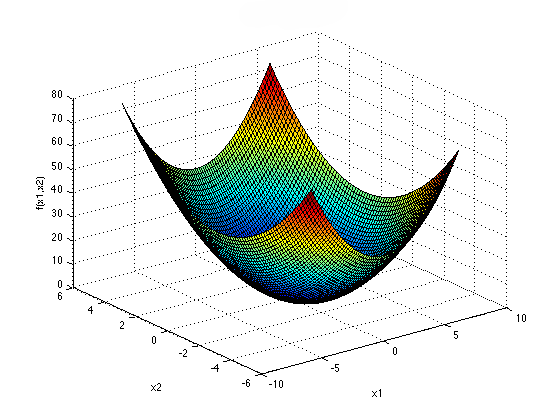
\includegraphics[width=\textwidth,height=\textheight,keepaspectratio]{sphere.png}
  \caption{Sphere's 2-dimensional graph function \cite{sf-uni-sp}}
\end{figure}

%%------------------------------------------------
 
\begin{table}[htbp]
\begin{minipage}{.4\linewidth}
    \centering

    \begin{tabular}{|c|c|c|c|c|}
    \hline
    D   & $\sigma$  & avg. time     & avg. sol.     & best sol. \\
    \hline
    10  & 0         & 89ms          & 0       & 0 \\
    \hline
    30  & 0         & 2.36s         & 0       & 0 \\
    \hline
    100 & 0         & 61.539s       & 0       & 0 \\
    \hline
    \end{tabular}
    \caption{Best improvement}
  \end{minipage}%
  \quad % ----------------------------------
  \begin{minipage}{.75\linewidth}
    \centering

    \begin{tabular}{|c|c|c|c|c|}
    \hline
    D   & $\sigma$  & avg. time     & avg. sol.     & best sol. \\
    \hline
    10  & 0         & 50ms          & 0             & 0 \\
    \hline
    30  & 0         & 1.21s         & 0             & 0 \\
    \hline
    100 & 0         & 32.58s        & 0             & 0 \\
    \hline
    \end{tabular}
    \caption{First improvement}
  \end{minipage}
\end{table}
\begin{table}[!htbp]
\begin{minipage}{.4\linewidth}
    \centering

    \begin{tabular}{|c|c|c|c|c|}
    \hline
    D   & $\sigma$  & avg. time     & avg. sol.     & best sol. \\
    \hline
    10  & 0         & 200ms         & 0             & 0 \\
    \hline
    30  & 0         & 4.98s         & 0             & 0 \\
    \hline
    \end{tabular}
    \caption{Worst improvement}
  \end{minipage}%
  \quad % ----------------------------------
  \begin{minipage}{.75\linewidth}
    \centering

    \begin{tabular}{|c|c|c|c|c|}
    \hline
    D   & $\sigma$  & avg. time     & avg. sol.     & best sol. \\
    \hline
    10  & 0         & 310ms         & 0             & 0 \\
    \hline
    30  & 0         & 4.97s         & 0             & 0 \\
    \hline
    100 & 0         & 152.95s       & 0             & 0 \\
    \hline
    \end{tabular}
    \caption{Simulated annealing}
  \end{minipage}
\end{table}

\newpage
\setcounter{table}{0}

%%------------------------------------------------

\subsection{Rastrigin}
$$ f(x) = A \cdot n + \sum_{i=1}^n \left[ x_i^2 - 10 \cdot cos(2 \pi x_i) \right] , x_i \in \left[ -5.12, 5.12 \right] $$

%%------------------------------------------------

\begin{figure}[!h]
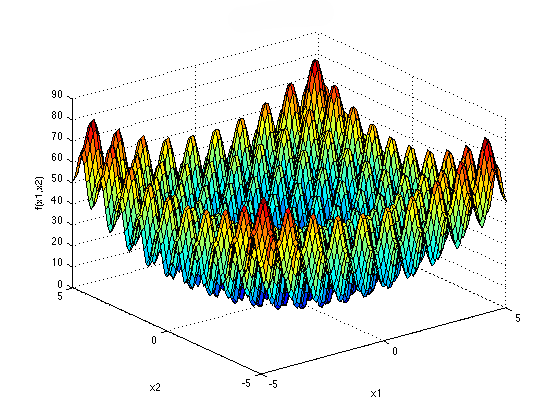
\includegraphics[width=\textwidth,height=\textheight,keepaspectratio]{rastrigin.png}
  \caption{Rastrigin's 2-dimensional graph function \cite{sf-uni-ra}}
\end{figure}

%%------------------------------------------------
    
\begin{table}[htbp]
\begin{minipage}{.4\linewidth}
    \centering
    
    \begin{tabular}{|c|c|c|c|c|}
    \hline
    D   & $\sigma$  & avg. time     & avg. sol.     & best sol.\\
    \hline
    10  & 0.53      & 307ms         & 1.96332       & 0.99496 \\
    \hline
    30  & 2.30      & 7.74s         & 22.49692      & 16.15900 \\
    \hline
    100 & 5.25      & 271.91s       & 124.04872     & 103.27991 \\
    \hline
    \end{tabular}
    \caption{Best improvement}
  \end{minipage}%
  \quad % ----------------------------------
  \begin{minipage}{.75\linewidth}
    \centering
    
    \begin{tabular}{|c|c|c|c|c|}
    \hline
    D   & $\sigma$  & avg. time     & avg. sol.     & best sol. \\
    \hline
    10  & 0.79      & 182ms         & 3.42327       & 1.23582 \\
    \hline
    30  & 2.63      & 4.37s         & 29.97694      & 22.84631 \\
    \hline
    100 & 4.99      & 154.12s       & 155.08213     & 141.60620 \\
    \hline
    \end{tabular}
    \caption{First improvement}
  \end{minipage}
\end{table}
\begin{table}[!htbp]
\begin{minipage}{.4\linewidth}
    \centering

    \begin{tabular}{|c|c|c|c|c|}
    \hline
    D   & $\sigma$  & avg. time     & avg. sol.     & best sol. \\
    \hline
    10  & 0.91      & 2.51s         & 5.12165       & 3.00004 \\
    \hline
    30  & 3.23      & 57.13s        & 38.18328      & 29.23457 \\
    \hline
    \end{tabular}
    \caption{Worst improvement}
  \end{minipage}%
  \quad % ----------------------------------
  \begin{minipage}{.75\linewidth}
    \centering

    \begin{tabular}{|c|c|c|c|c|}
    \hline
    D   & $\sigma$  & avg. time     & avg. sol.     & best sol. \\
    \hline
    10  & 0         & 19.81s        & 0       & 0 \\
    \hline
    30  & 0.86      & 171.31s       & 6.20453       & 3.99499 \\
    \hline
    100 & 1.94      & 19.16min      & 47.64466      & 40.26256 \\
    \hline
    \end{tabular}
    \caption{Simulated annealing}
  \end{minipage}
\end{table}

\newpage
\setcounter{table}{0}

%%------------------------------------------------

\subsection{Schwefel}
$$f(\mathbf{x}) = -\sum_{i=1}^{n} x_i \cdot \sin\left(\sqrt{|x_i|}\right) , x_i \in \left[-500,500\right]$$

%%------------------------------------------------

\begin{figure}[!h]
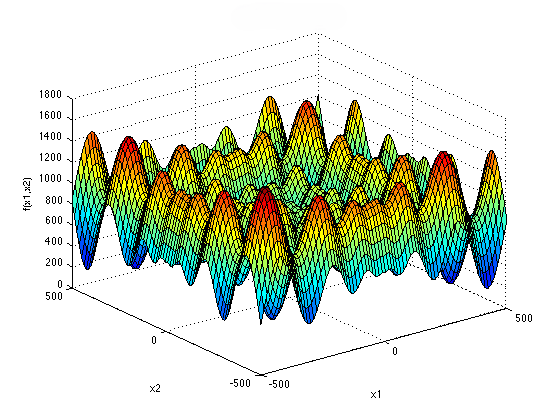
\includegraphics[width=\textwidth,height=\textheight,keepaspectratio]{schwefel.png}
  \caption{Schwefel's 2-dimensional graph function \cite{sf-uni-sw}}
\end{figure}
\vspace{0.5cm}

%%------------------------------------------------

\begin{table}[htbp]
\begin{minipage}{.4\linewidth}
    \centering

    \begin{tabular}{|c|c|c|c|c|}
    \hline
    D   & $\sigma$  & avg. time     & avg. sol.     & best sol. \\
    \hline
    10  & 18.4      & 755ms         & 17.70524      & 0.20936 \\
    \hline
    30  & 98.35     & 19.813s       & 894.62572     & 696.92139 \\
    \hline
    100 & 230.35    & 7,62min       & 5747.60089    & 5326.42004 \\
    \hline
    \end{tabular}
    \caption{Best improvement}
  \end{minipage}%
  \quad % ----------------------------------
  \begin{minipage}{.75\linewidth}
    \centering

    \begin{tabular}{|c|c|c|c|c|}
    \hline
    D   & $\sigma$  & avg. time     & avg. sol.     & best sol. \\
    \hline
    10  & 45.79     & 434ms         & 120.65099     & 34.54979 \\
    \hline
    30  & 111.23    & 11.18s        & 1464.46143    & 1186.97187 \\
    \hline
    100 & 217.08    & 261.82s       & 7615.11165    & 6976.11061 \\
    \hline
    \end{tabular}
    \caption{First improvement}
  \end{minipage}
\end{table}
\begin{table}[!htbp]
\begin{minipage}{.4\linewidth}
    \centering

    \begin{tabular}{|c|c|c|c|c|}
    \hline
    D   & $\sigma$  & avg. time     & avg. sol.     & best sol. \\
    \hline
    10  & 17.35     & 7.59s         & 212.34472     & 161.40279 \\
    \hline
    30  & 108.91    & 118.25s       & 1550.94308    & 1262.86526 \\
    \hline
    \end{tabular}
    \caption{Worst improvement}
  \end{minipage}%
  \quad % ----------------------------------
  \begin{minipage}{.75\linewidth}
    \centering

    \begin{tabular}{|c|c|c|c|c|}
    \hline
    D   & $\sigma$  & avg. time     & avg. sol.     & best sol. \\
    \hline
    10  & 0         & 22.98s        & 0.00037       & 0.00014 \\
    \hline
    30  & 0.07      & 173.01s       & 0.38921       & 0.21216 \\
    \hline
    100 & 41.02     & 25.93min      & 126.46816     & 71.91137 \\
    \hline
    \end{tabular}
    \caption{Simulated annealing}
  \end{minipage}
\end{table}

\newpage
\setcounter{table}{0}

%%------------------------------------------------

\subsection{Michalewicz}
$$f(\mathbf{x}) = -\sum_{i=1}^{n} \sin(x_i) \cdot \left(\sin\left(ix_i^2 / \pi\right)\right)^{2m} , m = 10, x_i \in \left[0,\pi\right]$$

%%------------------------------------------------

\begin{figure}[!h]
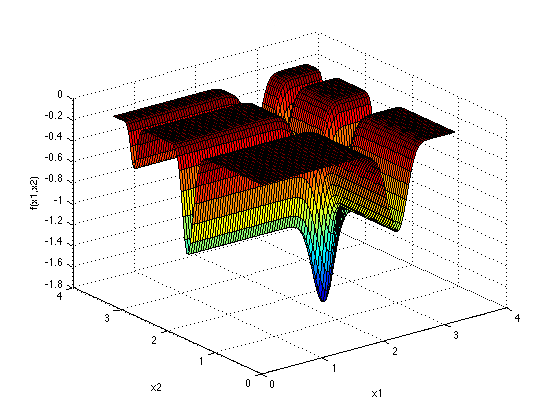
\includegraphics[width=\textwidth,height=\textheight,keepaspectratio]{michalewicz.png}
  \caption{Michalewicz's 2-dimensional graph function \cite{sf-uni-mc}}
\end{figure}
\vspace{0.5cm}

%%------------------------------------------------

\begin{table}[htbp]
\begin{minipage}{.4\linewidth}
    \centering

    \begin{tabular}{|c|c|c|c|c|}
    \hline
    D   & $\sigma$  & avg. time     & avg. sol.     & best sol. \\
    \hline
    10  & 0.04      & 1.50s         & -9.56506      & -9.65221 \\
    \hline
    30  & 0.28      & 33.42s        & -27.61249     & -28.56555 \\
    \hline
    100 & 0.51      & 9.73min       & -88.04727     & -89.11685 \\
    \hline
    \end{tabular}
    \caption{Best improvement}
  \end{minipage}%
  \quad % ----------------------------------
  \begin{minipage}{.75\linewidth}
    \centering

    \begin{tabular}{|c|c|c|c|c|}
    \hline
    D   & $\sigma$  & avg. time     & avg. sol.     & best sol. \\
    \hline
    10  & 0.05      & 865ms         & -9.50893      & -9.61160 \\
    \hline
    30  & 0.18      & 19.48s        & -27.02483     & -27.45056 \\
    \hline
    \end{tabular}
    \caption{First improvement}
  \end{minipage}
\end{table}
\begin{table}[!htbp]
\begin{minipage}{.4\linewidth}
    \centering

    \begin{tabular}{|c|c|c|c|c|}
    \hline
    D   & $\sigma$  & avg. time     & avg. sol.     & best sol. \\
    \hline
    10  & 0.12      & 7.39s         & -9.22340      & -9.42528 \\
    \hline
    30  & 0.29      & 104.44s       & -24.57051     & -25.19599 \\
    \hline
    \end{tabular}
    \caption{Worst improvement}
  \end{minipage}%
  \quad % ----------------------------------
  \begin{minipage}{.75\linewidth}
    \centering

    \begin{tabular}{|c|c|c|c|c|}
    \hline
    D   & $\sigma$  & avg. time     & avg. sol.     & best sol. \\
    \hline
    10  & 0         & 24.69s        & -9.65930      & -9.66015 \\
    \hline
    30  & 0.07      & 210.07s       & -29.11762     & -29.27980 \\
    \hline
    100 & 0.17      & 37.3min       & -95.99791     & -96.32860 \\
    \hline
    \end{tabular}
    \caption{Simulated annealing}
  \end{minipage}
\end{table}

%%------------------------------------------------

\section{Conclusions}

\subparagraph{}
Looking into our results, it can safely be stated that the Hill Climbing algorithm is efficient and succeeds in delivering significant values, in the search for the global minimum. Comparing it with the deterministic approach, the time is much less than the brute-force traversal of the graph function. The different improvement settings showcase diverse trade-offs between these designs which can be further exploited. \\

An exemplary observation would be the Simulated annealing contributions; they usually bring better solutions that are scalable for real competitive environments. It's useful in concrete cases, even though considerable time intervals were detected. \\

Overall, this study provides valuable insights into the application of optimization algorithms in solving complex optimization problems and contributes to the understanding of their performance across different dimensions. 

%%------------------------------------------------
%% bibliography

\begin{thebibliography}{9}

\bibitem{course}
  Croitoru Eugen - course \\ Hill Climbing documentation.
  \url{https://profs.info.uaic.ro/eugen.croitoru/teaching/ga/}

\bibitem{cuda}
  Nvidia Cuda coalesced memory \\
  \url{https://docs.nvidia.com/cuda/cuda-c-best-practices-guide/index.html\# coalesced-access-to-global-memory}

\bibitem{sf-uni-sp}
  Simon Fraser University \\ Sphere's function.
  \url{https://www.sfu.ca/~ssurjano/spheref.html}

\bibitem{sf-uni-ra}
  Simon Fraser University \\  Rastrigin's function.
  \url{https://www.sfu.ca/~ssurjano/rastr.html}

\bibitem{sf-uni-sw}
  Simon Fraser University \\ Schwefel's function.
  \url{https://www.sfu.ca/~ssurjano/schwef.html}

\bibitem{sf-uni-mc}
  Simon Fraser University \\ Michalewicz's function.
  \url{https://www.sfu.ca/~ssurjano/michal.html}


\end{thebibliography}  
\end{document}
